\documentclass[aspectratio=169,10pt]{beamer}
\usetheme{default}
\usepackage{amsmath,amssymb}
\usepackage{xcolor}
\usepackage{tikz}
\usetikzlibrary{arrows.meta,positioning,fit,backgrounds}
\setbeamertemplate{navigation symbols}{}
\definecolor{struc}{rgb}{0.10,0.32,0.55}
\setbeamercolor{structure}{fg=struc}
\setbeamerfont{frametitle}{size=\large}

\definecolor{geo}{rgb}{0.72,0.16,0.16}
\definecolor{learn}{rgb}{0.10,0.32,0.55}
\definecolor{frozen}{rgb}{0.42,0.42,0.42}

\newcommand{\Geo}[1]{\textcolor{geo}{#1}}
\newcommand{\Learn}[1]{\textcolor{learn}{#1}}

\title{Forward-Operator Attention}
\subtitle{Geometry-conditioned 3D localisation from projections}
\date{}

\begin{document}

% ======================================================================
\begin{frame}{The mechanism: one added term in one attention layer}
\vspace{-1mm}
\begin{columns}[T,onlytextwidth]
\begin{column}{0.54\textwidth}
\footnotesize
\textbf{1. Slots} \hfill\Learn{learned} + \Geo{fixed}\\[0.5mm]
$M$ embeddings $S\in\mathbb{R}^{M\times D}$ on a coarse grid of
\Geo{fixed mm coordinates} $\{p_m\}$ over the volume
($M=6^3=216$).

\medskip
\textbf{2. The gather} \hfill one cross-attention layer\\[0.5mm]
Queries $=$ slots. Keys/values $=$ \textcolor{frozen}{frozen}
vision-tower patches from all views, concatenated ($P=V\!\times\!324$).
\[
A \;=\; \mathrm{softmax}\!\Big(\tfrac{QK^{\!\top}}{\sqrt{d}}
   \;\Geo{+\;\tfrac{1}{\tau}\log w}\Big)
\]
\Geo{$w_{m,j}$}: does patch $j$ image the point $p_m$? From the
validated geometry kernel --- \emph{not learned}.

\medskip
\textbf{3. Conditioning tensor} \hfill 12 numbers/slot\\[0.5mm]
\[
N_m=\sum_{v} w_{m,v}\, d_{m,v} d_{m,v}^{\!\top},
\qquad d_{m,v}=\widehat{p_m - s_v}
\]
Eigendecompose the $3\!\times\!3$; the 3 eigenvalues and 3
eigenvectors go through a small MLP into the slot.

\medskip
\textbf{4. Wiring}\\[0.5mm]
Slots $\to$ \Learn{zero-init} linear $\to$ prepended to Qwen3-VL in
place of image tokens. LoRA the LM, freeze the tower.
\end{column}

\begin{column}{0.44\textwidth}
\centering
\vspace{1mm}
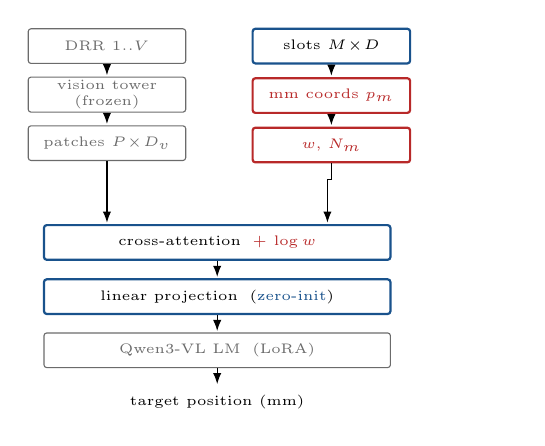
\begin{tikzpicture}[
  font=\tiny,
  box/.style={draw,rounded corners=1pt,minimum height=4.4mm,
              minimum width=20mm,align=center,inner sep=1pt},
  fz/.style={box,draw=frozen,text=frozen},
  ln/.style={box,draw=learn,thick},
  gg/.style={box,draw=geo,thick,text=geo},
  ar/.style={-{Latex[length=1.4mm]},shorten >=0.5pt}]

\node[fz] (v1) at (-1.35,0) {DRR $1..V$};
\node[fz,below=1.6mm of v1] (vt) {vision tower\\(frozen)};
\node[fz,below=1.6mm of vt] (pt) {patches $P\!\times\!D_v$};

\node[ln] (sl) at (1.5,0) {slots $M\!\times\!D$};
\node[gg,below=1.6mm of sl] (mm) {mm coords $p_m$};
\node[gg,below=1.6mm of mm] (ww) {$w$, $N_m$};

\node[ln,below=8mm of pt,xshift=14mm,minimum width=44mm] (ga)
  {cross-attention \;\Geo{$+\,\log w$}};
\node[ln,below=2.2mm of ga,minimum width=44mm] (pr)
  {linear projection \;(\Learn{zero-init})};
\node[fz,below=2.2mm of pr,minimum width=44mm] (lm)
  {Qwen3-VL LM \;(LoRA)};
\node[below=2.2mm of lm,font=\tiny] (out) {target position (mm)};

\draw[ar] (v1) -- (vt);
\draw[ar] (vt) -- (pt);
\draw[ar] (pt.south) -- ++(0,-2mm) -| ([xshift=-14mm]ga.north);
\draw[ar] (sl.south) -- (mm.north);
\draw[ar] (mm.south) -- (ww.north);
\draw[ar] (ww.south) -- ++(0,-2mm) -| ([xshift=14mm]ga.north);
\draw[ar] (ga) -- (pr);
\draw[ar] (pr) -- (lm);
\draw[ar] (lm) -- (out);

\node[right=0.5mm of ga,font=\tiny,text=geo,align=left,xshift=13mm]
  {};
\end{tikzpicture}

\vspace{1mm}
{\tiny \Geo{red = geometry, fixed} \quad \Learn{blue = learned} \quad
\textcolor{frozen}{grey = frozen}}
\end{column}
\end{columns}
\end{frame}

% ======================================================================
\begin{frame}{Why the two geometric terms do different jobs}
\footnotesize
\begin{columns}[T,onlytextwidth]
\begin{column}{0.49\textwidth}
\textbf{$\log w$ restricts \emph{where} a slot may look.}

\smallskip
A slot at $p_m$ can only attend to patches that physically image
$p_m$. The forward operator is imposed, not learned.

\smallskip
\begin{tabular}{@{}ll@{}}
$w$ density (2 views) & $1.9\%$ of $648$ patches\\
attention off-support & $0.00\mathrm{e}{+}00$\\
effective width $\tau\!=\!4$ & $36.4$ patches\\
\quad $\tau\!=\!1$ & $12.4$ patches\\
\quad $\tau\!=\!0.25$ & $4.8$ patches\\
uniform $w$ (ablation) & $648$ patches
\end{tabular}

\smallskip
$\tau$ anneals $4\!\to\!1$: sharp from step one gives dead gradients.
A slot no view can see is gated to zero --- otherwise softmax over an
all-masked row is \emph{uniform} and the slot would inject an average
of the whole image.

\medskip
\textbf{Cost.} $w$ depends only on geometry, so it is computed once
per (volume, view-set) and cached --- never during training.
\end{column}

\begin{column}{0.49\textwidth}
\textbf{$N_m$ tells the slot \emph{what its evidence cannot say}.}

\smallskip
$N_m=\sum_v w_{m,v} d_{m,v}d_{m,v}^{\!\top}$ is an outer-product sum
over the rays that image $p_m$, so its spectrum counts independent
directions of evidence:

\smallskip
\begin{tabular}{@{}lll@{}}
views & eigenvalues & rank\\
\hline
1 (PA) & $[1,\,0,\,0]$ & 1\\
2 (PA\,+\,LAT) & $[1.02,\,0.98,\,0]$ & 2\\
\end{tabular}

\smallskip
For one view the dominant eigenvector \emph{is} the ray
($|\cos|=1.000000$): the direction the view cannot resolve. Adding an
orthogonal view removes it.

\medskip
\textbf{Why this matters.} In-plane position lies in the
\emph{range} space of the projection and is recoverable from one view;
depth along the ray lies in the \emph{null} space and is not. $N_m$
hands the slot that distinction explicitly, rather than asking it to
infer the geometry from pixels.

\medskip
\textbf{Gate before any claim.} FOA vs.\ uniform $w$, same data, same
budget. If $\log w$ does not beat uniform, the mechanism is not doing
the work.
\end{column}
\end{columns}
\end{frame}

\end{document}
